\chapter{Algorithms for One-Dimensional Optimization}
\label{sec:algOneDimOpt}
\section{Interval Division Algorithms}
\lab{sec:IntDivAlg}
Interval division algorithm can be used to minimize a function $f \colon \Re \to \Re$,
(i.e., the function depends on one independent parameter only,)
over a user-specified interval.
The algorithms do not require derivatives and 
they require only one function evaluation per interval division, 
except for the initialization.

First, we explain a master algorithm for the interval division algorithms.
The master algorithm is used to implement two commonly used interval division algorithms: 
The Golden Section search and the Fibonacci Division. 

\begin{figure}
\centering
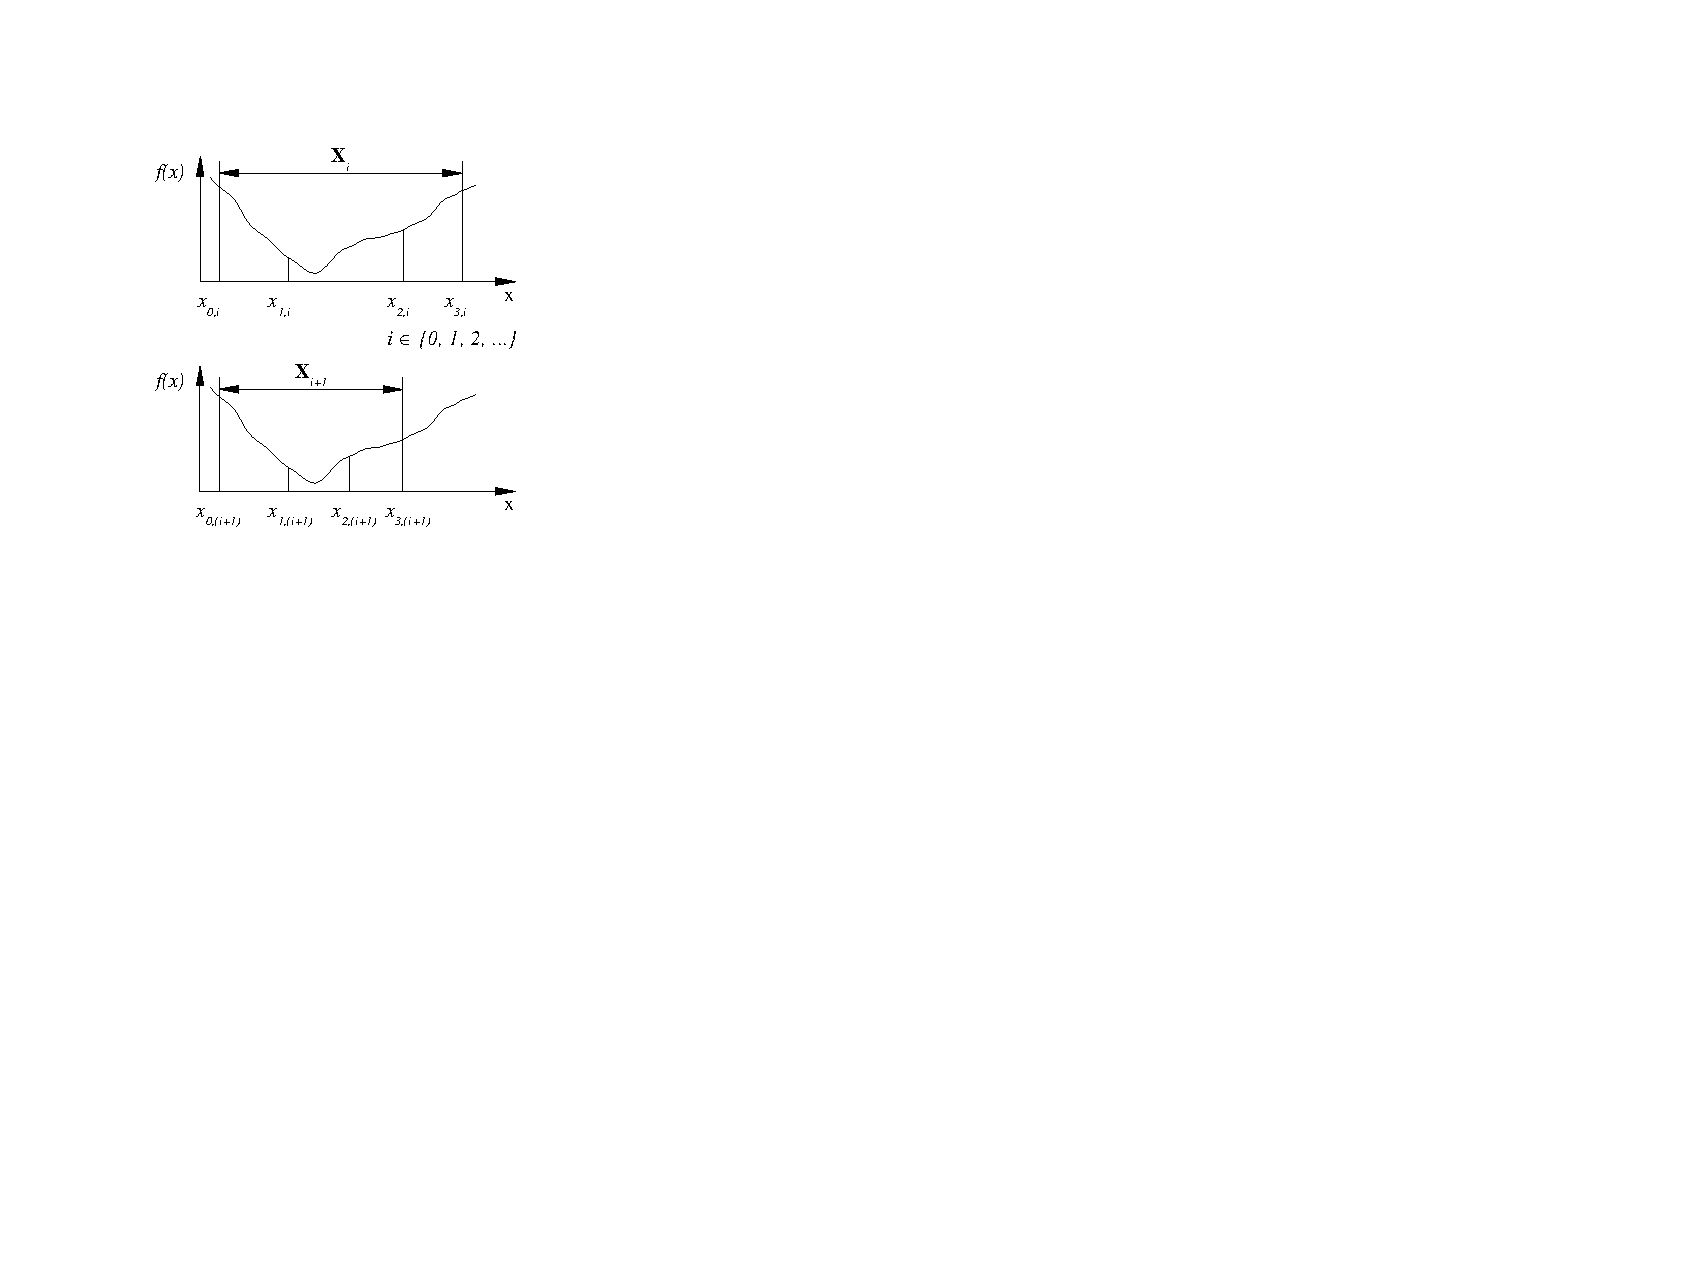
\epsfig{file=img/int_div.eps, bb=65 345 245 535}
\caption{Interval division.}
\label{fig:intDivGen}
\end{figure}

% --------
\subsection{General Interval Division}
We now describe the ideas behind the interval division methods.
For given $x_0, x_3 \in \Re$, with $x_0 < x_3$,
let $\mathbf X \triangleq [x_0, x_3]$.
Suppose we want to minimize $f(\cdot)$ on $\mathbf X$,
and suppose that $f \colon \Re \rightarrow \Re$ has a unique minimizer 
$x^* \in \mathbf X$.
For some $s \in (0, 1)$, let
\begin{eqnarray}
   x_1 & \triangleq & x_0 + s \, (x_3 - x_0), \\
   x_2 & \triangleq & x_1 + s \, (x_3 - x_1).
\end{eqnarray}
If $f(x_1) \le f(x_2)$, then $x^* \in  [x_0, \, x_2]$.
Hence, we can eliminate the interval $(x_2, \, x_3]$ 
and restrict our search to $[x_0, \, x_2]$.
Similarly, if $f(x_1) > f(x_2)$, then $x^* \in [x_1, \, x_3]$ 
and we can eliminate $[x_0, \, x_1)$.
Thus, we reduced the initial interval to a new interval that contains the minimizer $x^*$.\\

Let $i \in \Na$ be the iteration number.
We want to nest the sequence of intervals
\begin{equation}
[x_{0,(i+1)}, \, x_{3,(i+1)}] \subset [x_{0,i}, \, x_{3,i}], \qquad i \in \{0, \, 1, \, 2, \, \ldots \},
\end{equation}
such that we have to evaluate $f\depd$ in each step at one new point only.
To do so, we assign the new bounds of the interval such that either 
$[x_{0,(i+1)}, \, x_{3,(i+1)}] = [x_{0,i}, \, x_{2,i}]$, or $[x_{0, (i+1)}, \, x_{3, (i+1)}] = [x_{1,i}, \, x_{3,i}]$, 
depending on which interval has to be eliminated. 
By doing so, we have to evaluate only one new point in the interval. 
It remains to decide where to locate the new point.
The Golden Section and Fibonacci Division differ in this decision.

% --------
\subsection{Golden Section Interval Division}
Suppose we have three points $x_0 < x_1 < x_3$ in $\mathbf X \subset \Re$
such that for some $q \in (0, 1)$, to be determined later,
\begin{subequations}
\begin{equation}
   \frac{ | x_0 - x_1 | }{ | x_0 - x_3 |  } = q.
   \label{eq:golSecQDef}
\end{equation}
Hence,
\begin{equation}
   \frac{ | x_1 - x_3 | }{ | x_0 - x_3 |  } = 1-q.
\end{equation}
\end{subequations}

Suppose that $x_2$ is located somewhere between $x_1$ and $x_3$ and define
the ratio
\begin{equation}
  w \triangleq \frac{ | x_1 - x_2 | }{ | x_0 - x_3 |  }.
\end{equation}
Depending on which interval is eliminated, the interval in the next iteration step will
either be of length 
$(q+w) \, | x_0 - x_3|$, 
or $(1-q)  \, | x_0 - x_3|$.
We select the location of $x_2$ such that the two intervals are of the same length. 
Hence,
\begin{subequations}
\begin{equation}
   q + w = 1 - q.
  \label{eq:golSecqw}
\end{equation}
Now, we determine the fraction $q$.
Since we apply the process of interval division recursively, we know by scale similarity that
\begin{equation}
   \frac{ w }{ 1 - q } = q.
   \label{eq:golSecq}
\end{equation}
\end{subequations}
\begin{subequations}
Combining (\ref{eq:golSecqw}) and (\ref{eq:golSecq}) leads to
\begin{equation}
   q^2 - 3 q + 1 = 0,
\end{equation}
with solutions
\begin{equation}
   q_{1,2} = \frac{3 \pm \sqrt{5}}{2}.
\end{equation}
Since $q < 1$ by (\ref{eq:golSecQDef}), the solution of interest is
\begin{equation}
   q = \frac{3 - \sqrt{5}}{2} \approx 0.382.
\end{equation}
\end{subequations}

The fractional distances $q \approx 0.382$ and $1-q \approx 0.618$ correspond to the so-called \emph{Golden Section}, which gives this algorithm its name.\\

Note that the interval is reduced in each step by the fraction $1-q$, i.e., we have \emph{linear convergence}. In the $m$-th iteration, we have
\begin{eqnarray}
   | x_{ 0, \, m} - x_{ 2, \, m} | & = &
   | x_{ 1, \, m} - x_{ 3, \, m} | =
   | x_{ 0, \, (m+1)} - x_{ 3, \, (m+1)} | \nonumber \\
 & = &
   (1-q)^{m+1} \,    | x_{ 0, \, 0} - x_{ 3, \, 0} |.
\end{eqnarray}
Hence, the required number of iterations, $m$, to reduce the initial interval of uncertainty $|x_{0, \,0} - x_{3, \, 0} |$ to at least a fraction $r$, defined as
\begin{equation}
   r \triangleq \frac{ | x_{ 0, \, m} - x_{ 2, \, m} | }
                { | x_{ 0, \, 0} - x_{ 3, \, 0} | }
    = \frac{ | x_{ 1, \, m} - x_{ 3, \, m} | }
                { | x_{ 0, \, 0} - x_{ 3, \, 0} | },
  \label{eq:golSecDefR}
\end{equation}
is given by
\begin{equation}
  m = \frac{\ln r}{ \ln (1-q)} - 1.
\end{equation}


% =======================
\subsection{Fibonacci Division}
Another way to divide an interval such that we need one function evaluation per iteration can be constructed as follows: Given an initial interval $[x_{0, \, i}, x_{3, \, i}]$ , $i=0$, we divide it into three segments symmetrically around its midpoint. Let $d_{1,\, i} < d_{2,\, i} < d_{3,\, i}$ denote the distance of the segment endpoints, measured from $x_{0, \,i}$. Then we have by symmetry $d_{3,\, i}=d_{1,\, i} + d_{2,\, i}$. By the bracket elimination procedure explained above, we know that we are eliminating a segment of length $d_{1,\, i}$. Therefore, our new interval is of length $d_{3,\, (i+1)}= d_{2,\, i}$. By symmetry we also have $d_{3,\, (i+1)}= d_{1,\, (i+1)} + d_{2,\, (i+1)}$. Hence, if we construct our segment length such that $d_{3,\, (i+1)} = d_{1,\, (i+1)} + d_{2,\, (i+1)}= d_{2,\, i}$ we can reuse one known point. Such a construction can be done by using \emph{Fibonacci} numbers, which are defined recursively by
\begin{subequations}
\begin{eqnarray}
  F_0 & \triangleq & F_1 \triangleq 1, \\
  F_i & \triangleq & F_{i-1} + F_{i-2}, \qquad i \in \{2, \, 3, \, \ldots \}.
\end{eqnarray}
\end{subequations}
The first few numbers of the Fibonacci sequence are $\{1, \, 1, \,  2, \, 3, \, 5, \, 8, \, 13, \, 21, \, \ldots \}$. The length of the intervals $d_{1,\, i}$ and $d_{2, \, i}$, respectively, are then given by
\begin{equation}
   d_{1, \, i} = \frac{F_{m-i} }{ F_{m-i+2} }, \quad
  d_{2, \, i} = \frac{F_{m-i+1} }{ F_{m-i+2} }, \qquad
  i \in \{0, \, 1, \, \ldots \, , \, m \},
\end{equation}
where $m > 0 $ describes how many iterations will be done. Note that $m$ must be known prior to the first interval division. 
Hence, the algorithm must be stopped after $m$ iterations.\\

The reduction of the length of the uncertainty interval per iteration is given by
\begin{equation}
  \frac{ d_{3, \, (i+1)} }{  d_{3, \, i}  } =
  \frac{ d_{2, \, i} }{  d_{1, \, i} + d_{2, \, i}  } = 
   \frac{  \frac{ F_{m-i+1} }{F_{m-i+2}}  }
     {  \frac{F_{m-i}}{F_{m-i+2}} +  \frac{F_{m-i+1}}{F_{m-i+2}}   } = 
        \frac{ F_{m-i+1}   }{ F_{m-i+2}   }.
\end{equation}
After $m$ iterations, we have
\begin{eqnarray}
  \frac{d_{3, \, m}}{d_{3, \, 0}} & = & 
  \frac{ d_{ 3, \, m}  }{ d_{ 3, \, (m-1)}  } \, 
  \frac{ d_{ 3, \, (m-1)}  }{ d_{ 3, \, (m-2)}  } \,
   \ldots \,
   \frac{ d_{ 3, \, 2}  }{ d_{ 3, \, 1}  } \,
   \frac{ d_{ 3, \, 1}  }{ d_{ 3, \, 0}  } \nonumber \\
 & = &
  \frac{F_{2} }{ F_{3} } \, 
  \frac{F_{3} }{ F_{4} } \, \ldots \, 
  \frac{F_{m} }{ F_{m+1} } \, 
  \frac{F_{m+1} }{ F_{m+2} } 
=
  \frac{2}{F_{m+2}}.
\end{eqnarray}
The required number of iterations $m$ to reduce the initial interval $d_{3, \, 0}$ 
to at least a fraction $r$, defined by (\ref{eq:golSecDefR}), can again be obtained by expansion from
\begin{eqnarray}
  r & = & 
  \frac{d_{2, \, m}}{d_{3, \, 0}} = 
  \frac{ d_{ 3, \, (m+1)}  }{ d_{ 3, \, 0}  } = 
  \frac{ d_{ 3, \, (m+1)}  }{ d_{ 3, \, m}  } \,
  \frac{ d_{ 3, \, m}  }{ d_{ 3, \, (m-1)}  } \,
   \ldots \,
   \frac{ d_{ 3, \, 2}  }{ d_{ 3, \, 1}  } \,
   \frac{ d_{ 3, \, 1}  }{ d_{ 3, \, 0}  } \, \nonumber \\
 & = &
  \frac{F_{1} }{ F_{2} } \, 
  \frac{F_{2} }{ F_{3} } \, \ldots \, 
  \frac{F_{m} }{ F_{m+1} } \, 
  \frac{F_{m+1} }{ F_{m+2} } 
=
  \frac{1}{F_{m+2}}.
\end{eqnarray}
Hence, $m$ is given by
\begin{equation}
  m = \argmin_{m \in \Na} \left\{ m \ | \ r \ge \frac{1}{F_{m+2}} \right\}.
\end{equation}


% -----------------
\subsection{Comparison of Efficiency}
The Golden Section is more efficient than the Fibonacci Division. Comparing the reduction of the interval of uncertainty, $| x_{0, \, m} - x_{3, \, m}|$, in the limiting case for $m \rightarrow \infty$, we obtain
\begin{equation}
   \lim_{m \rightarrow \infty} \frac{ | x_{0, \, m} - x_{3, \, m}  |_{GS} }
  { | x_{0, \, m} - x_{3, \, m}  |_{F} }
= \lim_{m \rightarrow \infty} \frac{F_{m+2}}{2} \, (1-q)^m = 0.95.
\end{equation}

% --------------------

\subsection{Master Algorithm for Interval Division}
The following master algorithm explains the steps of 
the interval division algorithm.\\

\noindent
\begin{minipage}[b]{\textwidth}
\begin{algorithm}
[Model Interval Division Algorithm]
~\\
{\em
\begin{tabularx}{\headwidth}{m{2cm}l}
\multicolumn{2}{l}{\hspace{\textwidth}~} \\ \\[-8ex]\\
\hline \\[-2ex]
 \textbf{Data}: 
 & $x_0$, $x_3$. \\
 & Procedure that returns $r_i$, defined as\\
 & $r_i \triangleq |x_{0, \, i} - x_{2, \, i} | / |x_{0, \, 0} - x_{3, \, 0}|$. \\
\textbf{Step 0:} 
 & {\it Initialize }\\
  & $\Delta x = x_3 - x_0$,\\
  &$ x_2 = x_0 + r_1 \, \Delta x$,\\
  & $x_1 = x_0 + r_2 \, \Delta x$,\\
  & $f_1 = f(x_1)$, $ f_2 = f(x_2)$, and\\
  & $i = 2$.\\
\textbf{Step 1:} & {\it Iterate.}\\
  & Replace $i$ by $i + 1$.\\
  & If  $(f_2 < f_1)$\\
    &  \hspace{1cm}  Set  $x_0 = x_1$, $x_1 = x_2$,\\
    &   \hspace{1cm}   $f_1 = f_2$,\\
    &   \hspace{1cm}   $x_2 = x_3 - r_i \, \Delta x$, and\\
    &    \hspace{1cm}  $f_2 = f(x_2)$.\\
   & else\\
   &    \hspace{1cm} Set $x_3 = x_2$, $x_2 = x_1$,\\
   &    \hspace{1cm}  $f_2 = f_1$,\\
   &    \hspace{1cm}  $x_1 = x_0 + r_i \,  \Delta x$,\\
   &    \hspace{1cm}  $f_1 = f(x_1)$.\\
   \textbf{Step 2:} & Stop or go to Step 1.\\
   \hline \\
\end{tabularx}
}
\lab{al:ModOneDim}
\end{algorithm}
\end{minipage}
% ---------------------

\subsection{Keywords}
For the Golden Section and the Fibonacci Division algorithm, the command file (see page~\pageref{par:comFil}) must contain only one continuous parameter.\\

To invoke the Golden Section or the Fibonacci Division algorithm, the \texttt{Algorithm} Section of the GenOpt command file must have following form:
\begin{lstlisting}
Algorithm{
   Main              = GoldenSection | Fibonacci;
  [AbsDiffFunction   = Double;  |   // 0 < AbsDiffFunction
   IntervalReduction = Double;  ]   // 0 < IntervalReduction
}
\end{lstlisting}
\pagebreak[2]
\noindent The keywords have the following meaning
\begin{codedescription}
\item[Main]
The name of the main algorithm.
\end{codedescription}
The following two keywords are optional. If none of them is specified, then the algorithm stops after \texttt{MaxIte} function evaluations (i.e., after \texttt{MaxIte}$-2$ iterations), where \texttt{MaxIte} is specified in the section \texttt{OptimizationSettings}. If both of them are specified, an error occurs.
\begin{codedescription}
\item[AbsDiffFunction]
The absolute difference defined as
\begin{equation}
\Delta f \triangleq | \min \{ f(x_0),\, f(x_3) \} - \min \{ f(x_1), \, f(x_2) \}|.
\end{equation}
If $\Delta f$ is lower than \texttt{AbsDiffFunction}, the search stops successfully.\\
\underline{Note:} Since the maximum number of interval reductions must be known for the initialization of the Fibonacci algorithm, this keyword can be used only for the Golden Section algorithm. It must not be specified for the Fibonacci algorithm.
\item[IntervalReduction]
The required maximum fraction, $r$, of the end interval length relative to the initial interval length (see equation~\eqref{eq:golSecDefR}).
\end{codedescription}
